\chapter{Optical Music Recognition}
\label{chap:OMR}

This chapter contains an introduction to optical music recognition (OMR). Most of its content is based on the article \emph{Understanding Optical Music Recognition} (\cite{UnderstandingOmr}).

The article defines OMR as \emph{a field of research that investigates how to computationally read music notation in documents}. This definition attempts to clearly define the term. OMR is a field of research, therefore it encapsualtes the investigation of many problems -- it is not a single task. OMR attempts to computationally read music; it applies existing understanding of various music notations and does not study these notations as such. Recognized documents may be of many types (scanned, digitally-engraved, printed, handwritten, captured from a stylus) and be represented in different music notations (common western, mensural, tablature). This thesis focuses on reading entire pages of handwritten music, expressed in the common western music notation.

The recognition process on its own is also not very useful. It serves as one phase of solving some larger problem, like metadata extraction, archive searching, audio replay, editing or conversion to some other music data format. Each one of these applications has a different set of priorities regarding the recognition. If the goal is to seach by melody, we do not need to recognize rhythm; if the goal is audio replay, we do not need to read lyrics.

It should be noted, that there is a difference between recovering musical semantics and recovering music notation. This stems from the specifics of how music notation encodes musical ideas. Musical symbols on a staff compete for space and this influences their relative position. In music notation, there is also a lot of freedom in how a musical idea is expressed. Some rhytmic phrases may be expressed using either duration dots or using ties and the choice may depend on the writer's preference or on the rhytmic context. Recovering music notation is the easier task of reading individual notation symbols and their relationships. Recovering musical semantics requires an additional step of interpreting the parsed musical notation.

\begin{figure}[ht]
    \centering
    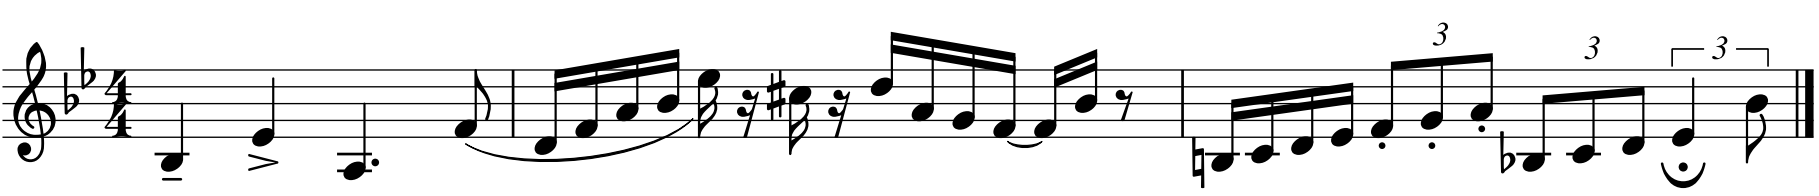
\includegraphics[width=145mm]{../img/music-monophonic.png}
    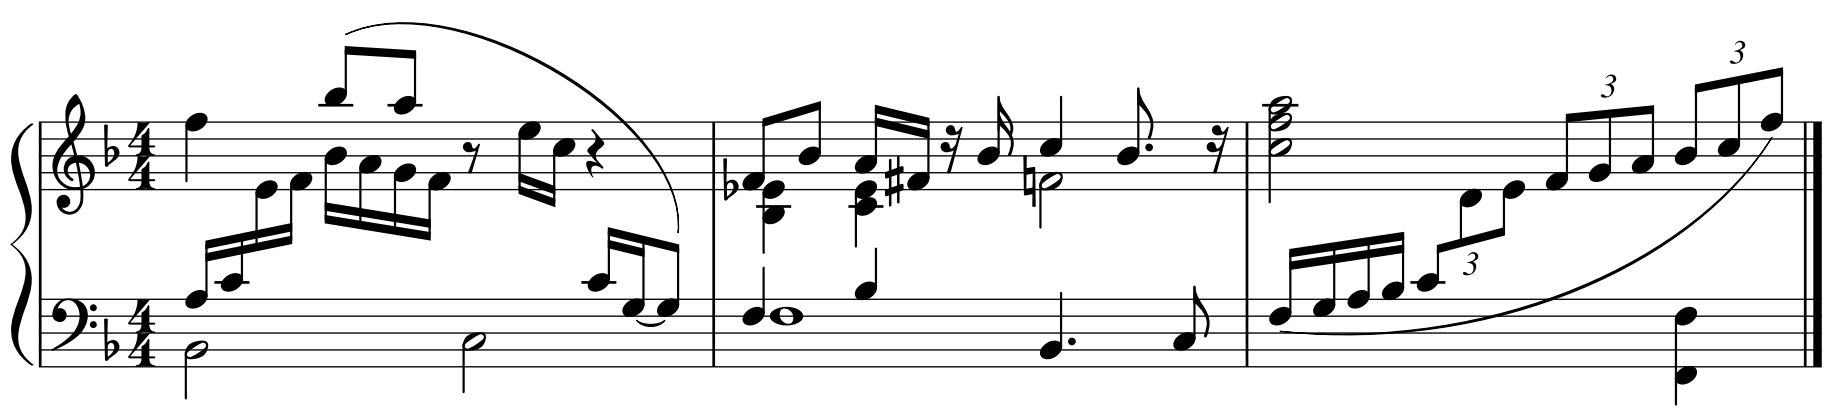
\includegraphics[width=145mm]{../img/music-pianoform.png}
    \caption{Comparison of monophonic music (top) to a pianoform (bottom). Monophonic music contains only a single voice and can be represented sequentially. Pianoform contains multiple voices spread out over two staves, making it behave more like a graph. The image is taken from (\cite{UnderstandingOmr}).}
    \label{fig:MusicComplexity}
\end{figure}

It is only natural to ask about the relationship of OMR and text recognition. Both fields attempt to read documents containing sequential data and there are many other similarities. However, music recognition is much more difficult for multiple reasons. Music notation is contextual, meaning that interpretation of some symbols depends on other symbols around it. Pitch of a note is one example. We need to know both the key signature (correctly read the clef and accidentals at the beggining of the staff) vertical note position (in relation to staff lines) and possibly an additional accidental in front of the notehead. Size and shape of symbols varies from very small (a dot) to relatively large (beams, slurs, hairpins) to spanning the entire page (tall barlines or braces). Lastly, a single staff of music can contain multiple voices and a pianoform may contain two to three voices on two staves and some notation symbols may be present on both staves simultaneously. Text recognition usually does not need to deal with such a level of complexity.


\section{Approaches to OMR}

Traditional recognition systems relied on the detection of individual symbols and their classification. Stafflines intersect the majority of all symbols, which posed a problem to most object detectors that relied on finding connected components. For this reason, staffline removal was an important preprocessing step.

In recent years, deep learning has been applied to many OMR problems with great success. Especially symbol classification and staffline removal have been considerably improved (\cite{StafflineDetection}, \cite{PachaClassification}). Convolutional neural networks are well capable of learning handwritten symbol classification despite the variance in handwriting styles. In fact, they are able to perform classification without the need for staffline removal -- aggregating multiple phases of a traditional pipeline and greatly simplifying the task.

The pipeline for music recognition has been refined over the years (\cite{BainbridgeBell}, \cite{RebeloSota}) and has currently reached a form with four distinct stages:

\begin{itemize}
    \item \textbf{Preprocessing} Methods that enhance the raw scanned or photographed document for easier processing. These contain perspective compensation, page cropping, contrast enhancement, binarization, noise removal. Basic layout analysis (such as staff detection) also belongs here.
    \item \textbf{Music Object Detection} Finding and classifying all notation symbols.
    \item \textbf{Notation Assembly} Identifying relations between detected symbols and constructing a machine-readable representation (a sequence or a graph).
    \item \textbf{Encoding} Reading and interpreting the recognised notation to fulfil the given task (conversion to another format, audio replay, ...).
\end{itemize}

The introduction of deep learning has allowed an alternative approach to be developed, where all of these stages are performed by a single model. This end-to-end approach has yielded state-of-the-art results in other fields, such as handwritten text recognition (\cite{Scheidl}). It has also been tried for music recognition (\cite{Primus}, \cite{Mayer}), but modelling the complex graph-like structure of music notation is problematic, and so this approach has been limited to monophonic music (which can be represented sequentially).

This thesis focuses on semantic segmentation, which is used as the first step of the object detection stage.


\section{Datasets}
\label{sec:Datasets}

With the shift towards machine learning, several datasets have been created to allow machine learning models to be trained. This thesis relies on three of these datasets:

\begin{itemize}
    \item CVC-MUSCIMA (\cite{CvcMuscima})
    \item MUSCIMA++ (\cite{MuscimaPP})
    \item DeepScores v2 (\cite{DeepScores})
\end{itemize}

These are the only datasets in the OMR field that contain semantic segmentation labels (for Common Western Music Notation). A comprehensive list of other available OMR datasets is maintained by Alexander Pacha on his GitHub page\footnote{\url{https://apacha.github.io/OMR-Datasets/}}.


\subsection{CVC-MUSCIMA}

\begin{figure}[ht]
    \centering
    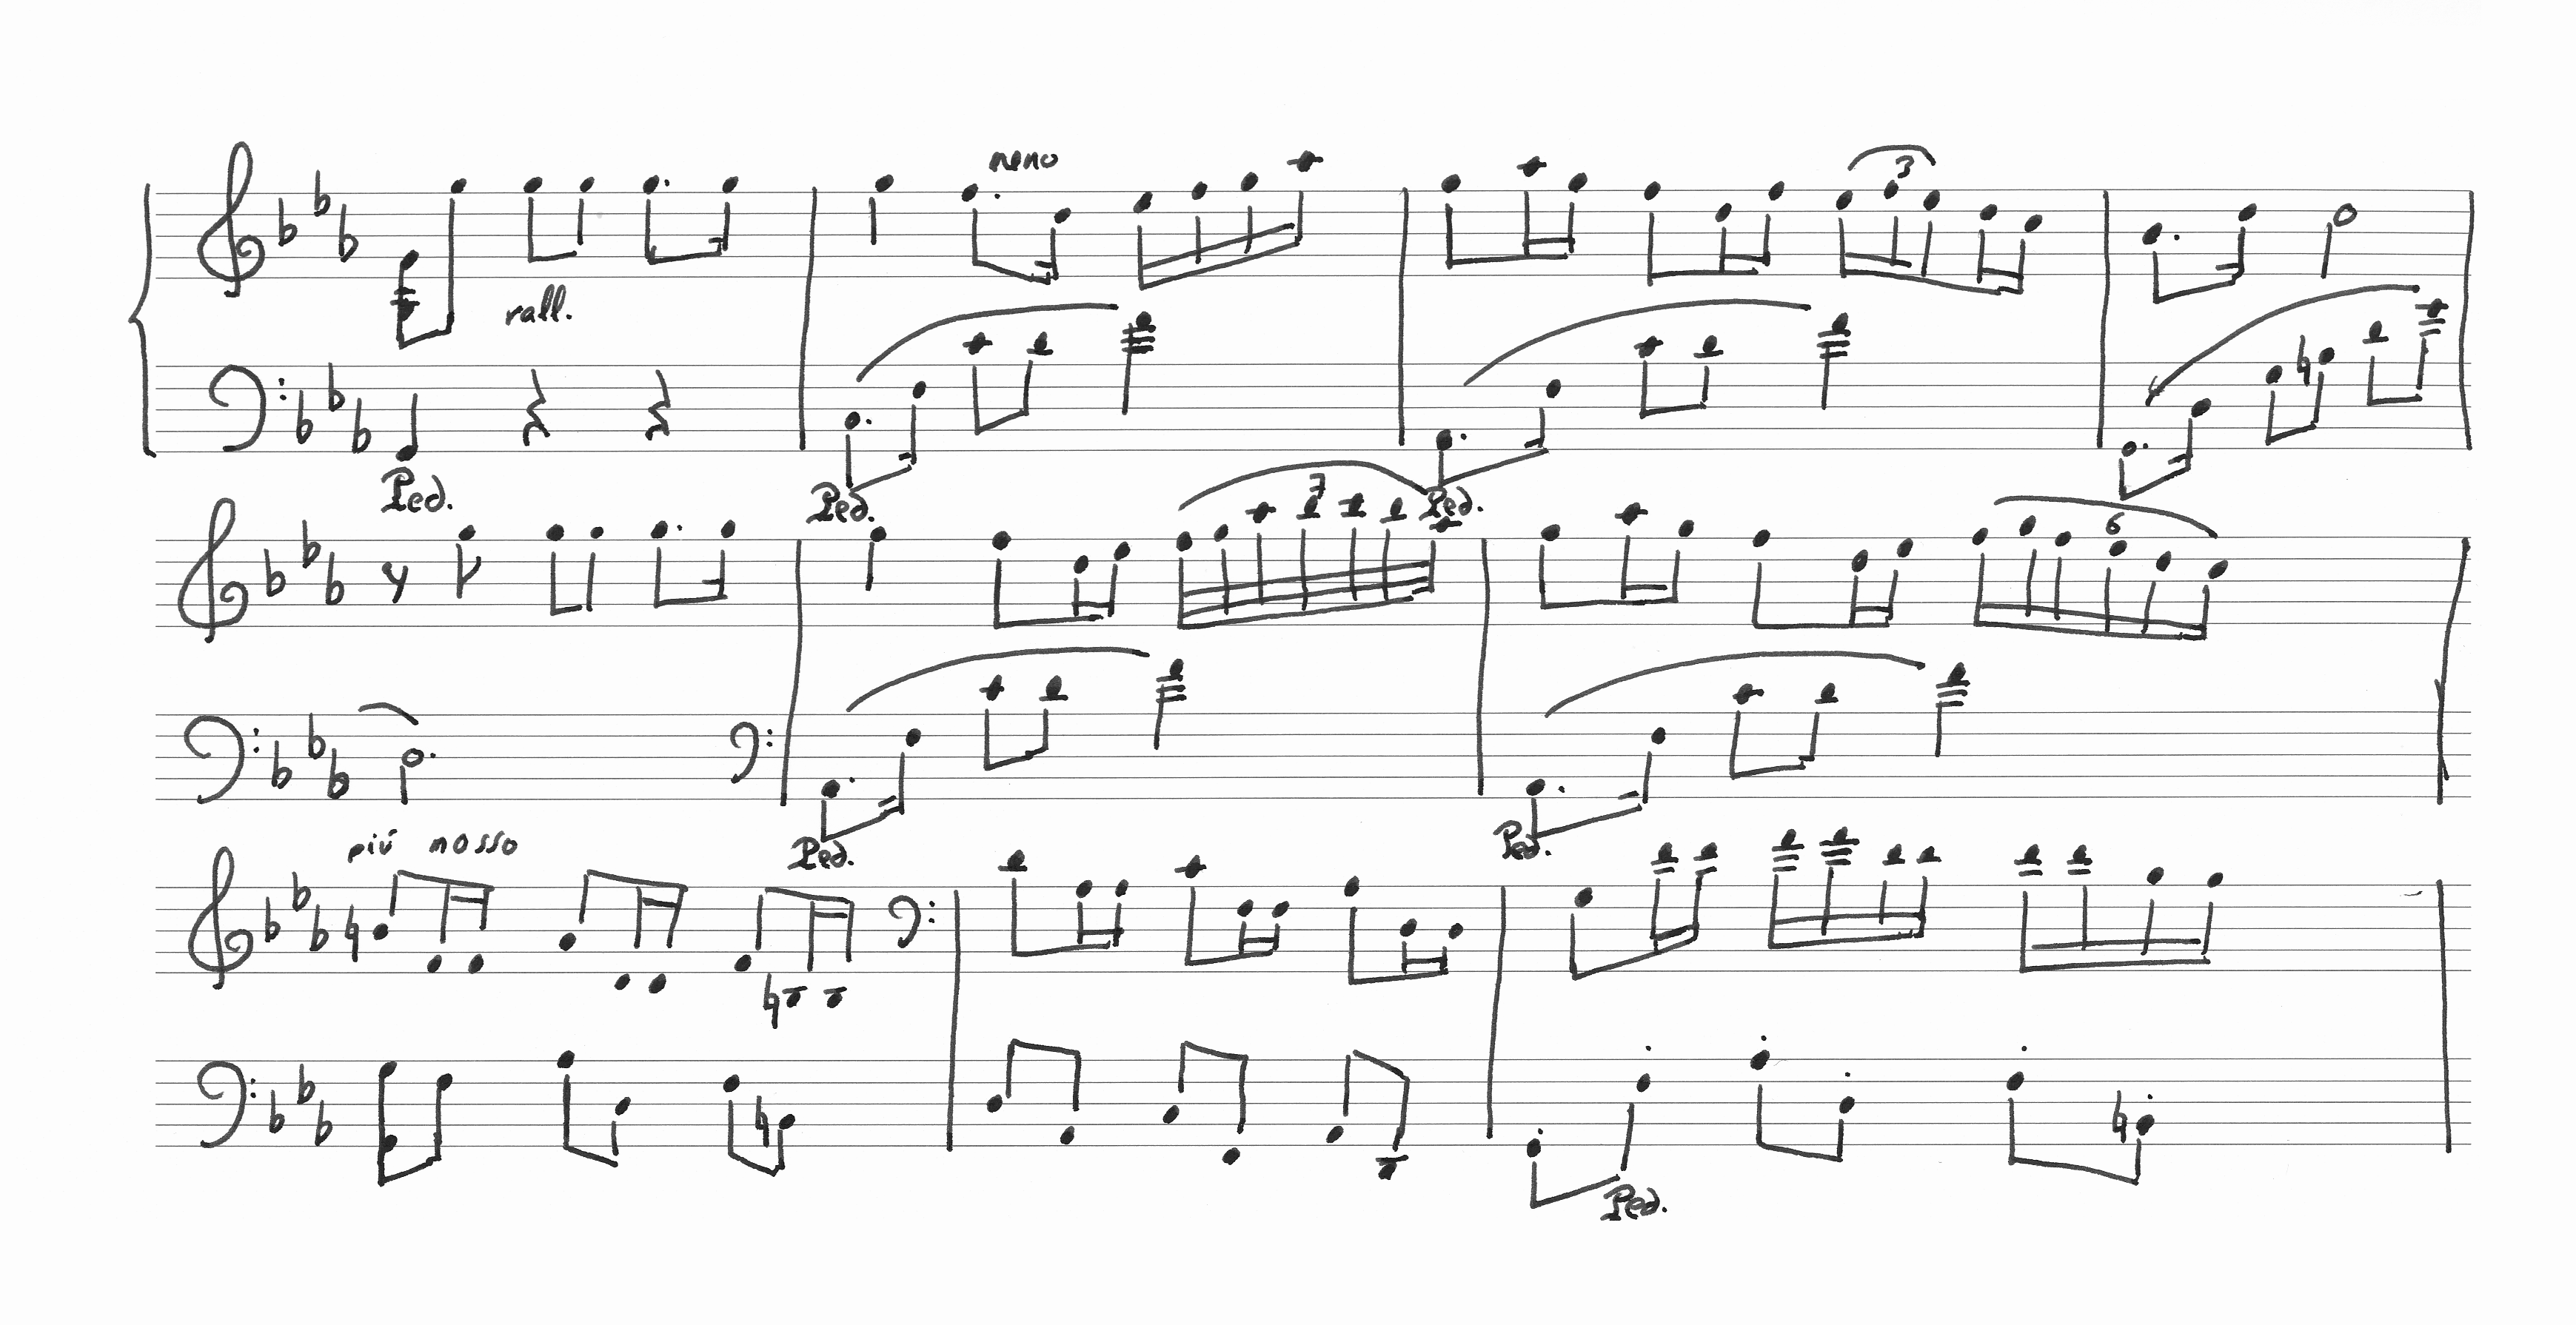
\includegraphics[width=145mm]{../img/cvc-muscima.png}
    \caption{One page from the CVC-MUSCIMA dataset. The image is taken from the website \url{http://www.cvc.uab.es/cvcmuscima/index_database.html}}
    \label{fig:CvcMuscima}
\end{figure}

This dataset was introduced in the article \emph{CVC-MUSCIMA: A ground truth of handwritten music score images for writer identification and staff removal} (\cite{CvcMuscima}). It contains 1000 pages of handwritten music, created by having 50 writers transcribe 20 unique music pages. It was designed for the tasks of staff removal and writer identification. It is also the only handwritten music dataset, consisting of entire music pages -- all other handwritten datasets contain only individual symbols. This makes it very important for research focusing on symbol detection.

Since the dataset does not contain segmentation labels, we will use it primarily as a source of unlabeled training data.


\subsection{MUSCIMA++}

MUSCIMA++ was created by Jan Hajič jr. and Pavel Pecina as a general-purpouse OMR dataset. It was introduced in the article \emph{In Search of a Dataset for Handwritten Optical Music Recognition: Introducing MUSCIMA++} (\cite{MuscimaPP}). The dataset builds on top of the CVC-MUSCIMA dataset, providing rich annotations for 140 selected pages. The annotation scheme was designed to be sufficiently low-level for tasks such as object detection (bounding boxes, symbol classes, segmentation masks), while also having relationship data in the form of an oriented graph, that lets a user extract semantic information about the music. Dataset authors call this annotation scheme the \emph{Music Notation Graph} (MuNG).

\begin{figure}[ht]
    \centering
    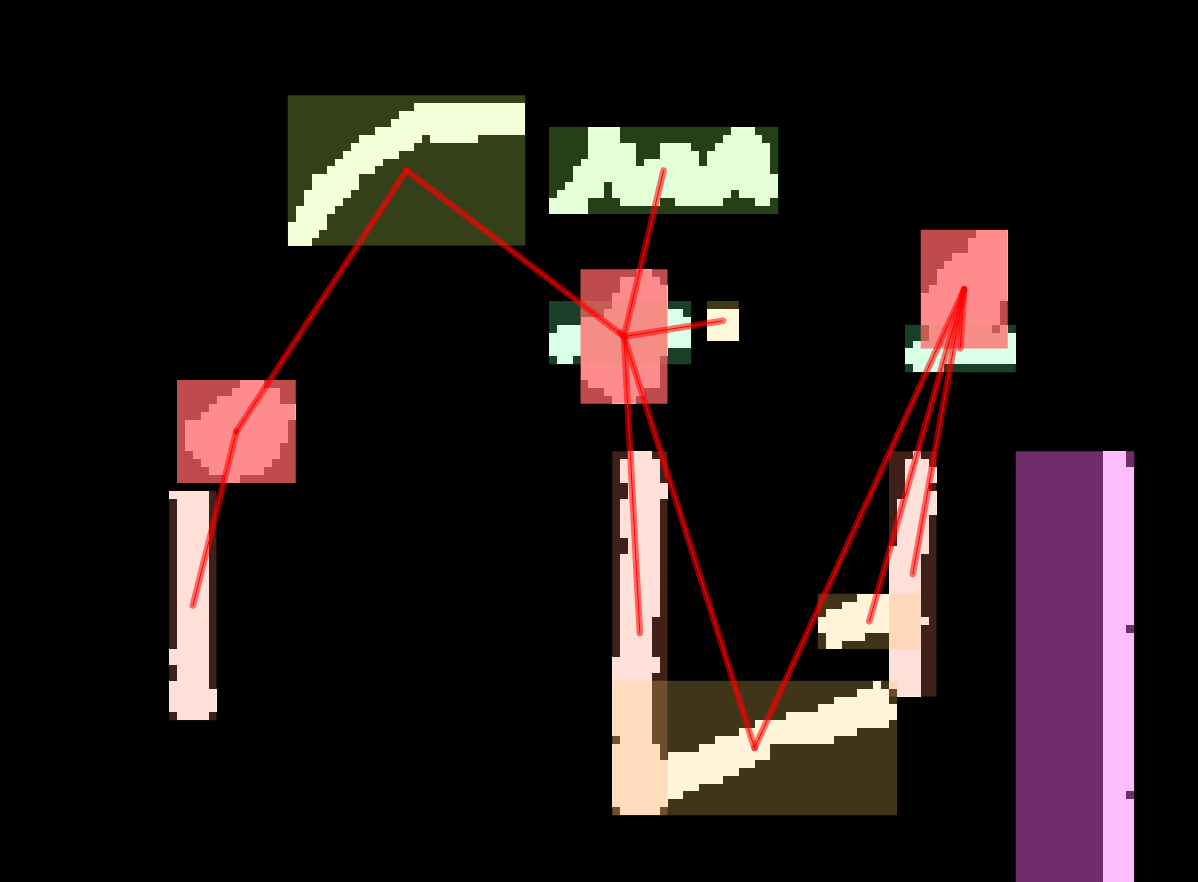
\includegraphics[width=70mm]{../img/muscima-pp.png}
    \caption{Annotations present in the MUSCIMA++ dataset (bounding boxes, segmentation masks and the notation graph). The image is taken from \cite{MuscimaPP}}
    \label{fig:MuscimaPP}
\end{figure}

The dataset was updated in 2019, fixing bugs and modifying class names to be aligned with the SMuFL\footnote{\url{https://www.smufl.org/}} standard. A similar update was also performed on the DeepScores dataset (\cite{DeepScores}), making it easier to use both datasets simultaneously. The latest dataset description and accompanying tools can be found on the GitHub page\footnote{\url{https://github.com/OMR-Research/muscima-pp}} of the OMR Research group\footnote{\url{https://omr-research.net/}}.

We will use this dataset as a source of labeled data for semantic segmentation.


\subsection{DeepScores}

The version 2 of this dataset was introduced in the article \emph{The DeepScoresV2 Dataset and Benchmark for Music Object Detection} (\cite{DeepScores}). The dataset contains entire pages of printed music, with annotations best suited for object detection, semantic segmentation and object classification. It was created from MusicXML documents taken from the MuseScore\footnote{\url{https://musescore.com/sheetmusic}} website and engraved using the LilyPond\footnote{\url{https://lilypond.org/}} tool. The dataset contains 255,386 pages of music, but also provides a dense and diverse subset, having only 1,714 pages. The version 2 also introduced a MUSCIMA++ compatibility mode, making it easier for the two datasets to be used simultaneously.

\begin{figure}[ht]
    \centering
    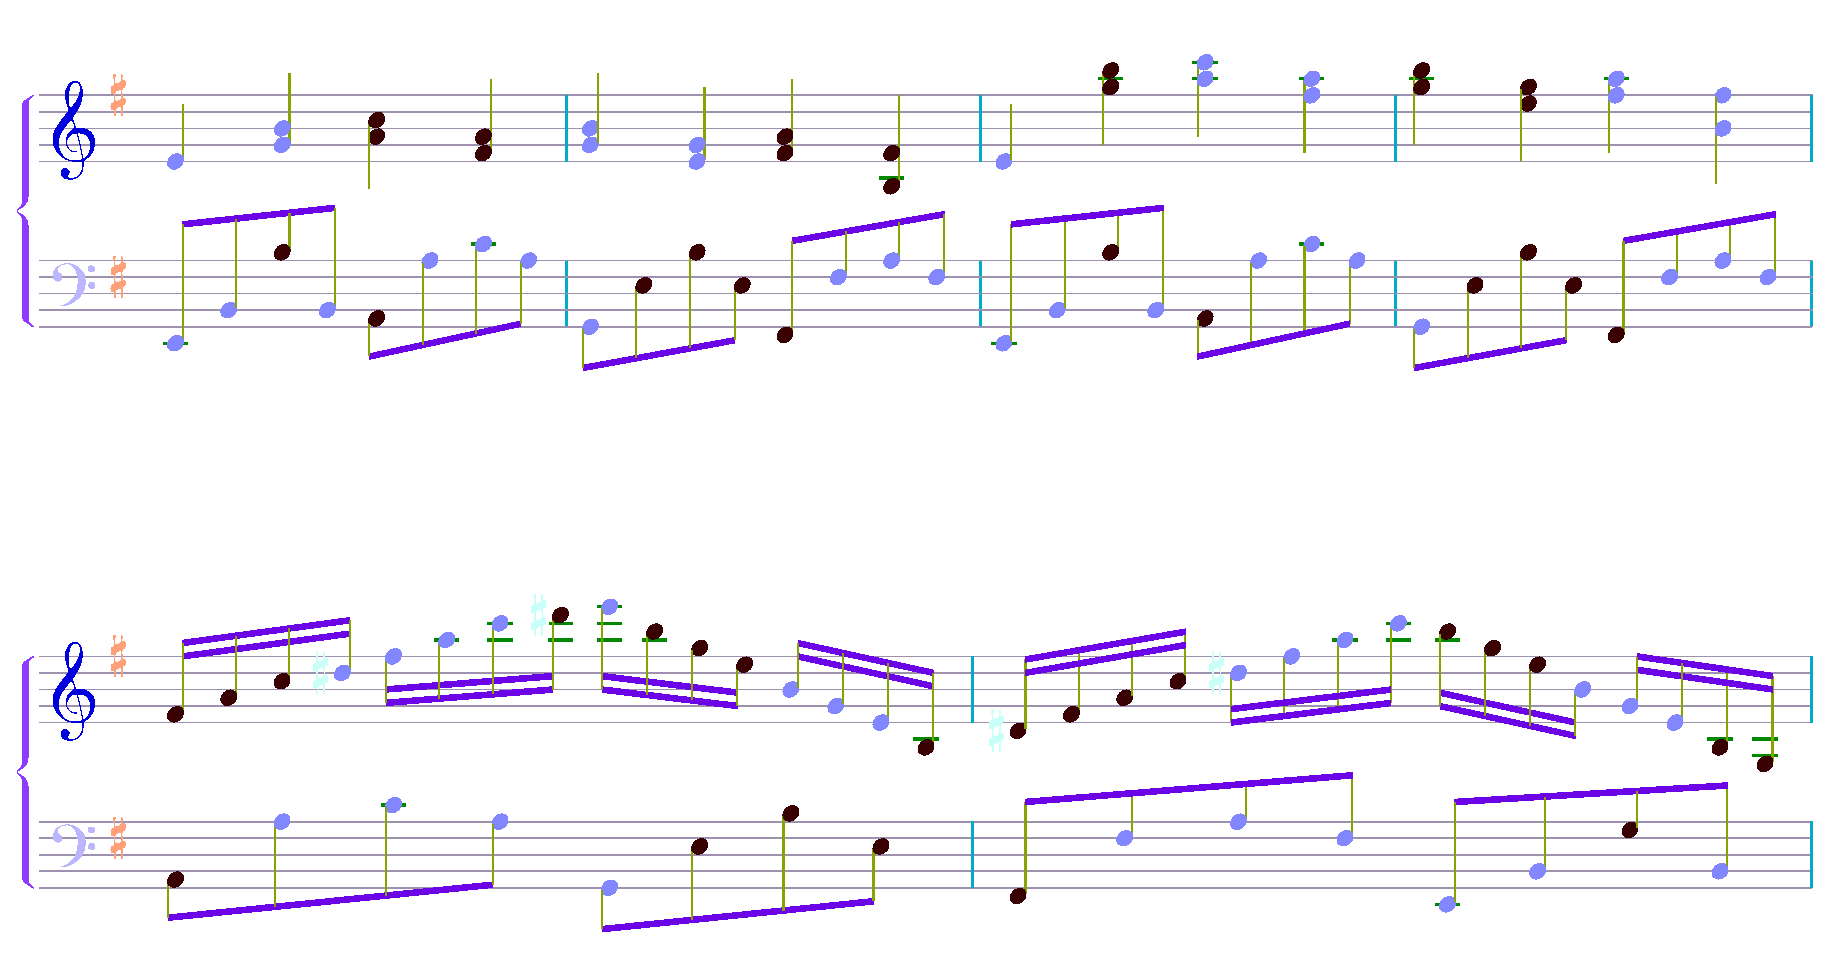
\includegraphics[width=145mm]{../img/deepscores.png}
    \caption{An example of semantic segmentation labels from the DeepScores v2 dataset. The dataset is very large, but digitally engraved.}
    \label{fig:DeepScoresV2}
\end{figure}

We will use this dataset as a source of labeled data for semantic segmentation.
